\documentclass[../../thesis]{subfiles}

\IfEq{\jobname}{\detokenize{thesis}}{}{%
    \setcounterref{chapter}{chap:implementation}
    \addtocounter{chapter}{-1}
}


\begin{document}

\chapter{Lập trình \& Kiểm thử}\label{chap:implementation}

Chương này nêu một số đoạn mã trong quá trình lập trình và kiểm thử, cùng với
ảnh chụp màn hình của kết quả cuối cùng.


%----------------------------------------------------------------------------------------
%	Lập trình
%----------------------------------------------------------------------------------------

\section{Lập trình}\label{sec:coding}

\subsection{Coroutine}

Về mặt lập trình, trong quá trình viết ứng dụng, một trong các khó khăn chủ yếu
là tăng tốc ứng dụng bằng coroutine. Trang sau trình bày một trong những đoạn mã
dùng coroutine trong ca sử dụng tìm kiếm, có sử dụng cả LiveData:

Đoạn mã đó trả về một đối tượng \texttt{LiveData<List<List<Metadata>>>}:

\begin{itemize}
    \item
        \texttt{Metadata}: Đối tượng chứa một kết quả tìm kiếm, có thể là
        \texttt{Comic}, \texttt{Series},\ldots{}
    \item
        \texttt{List<Metadata>}: Chứa kết quả tìm kiếm của một DAO, các
        \texttt{Metadata} trong danh sách này thuộc cùng một kiểu.
    \item
        \texttt{List<List<Metadata>>}: Danh sách kết quả của một DAO, nếu có kết
        quả (không rỗng) sẽ được thêm vào danh sách tổng hợp. Danh sách tổng hợp
        chính là danh sách kết quả tìm kiếm \emph{chưa làm phẳng} (xem lại
        \hyperref[sec:search-comic]{ca sử dụng tìm kiếm} về cách làm phẳng).
    \item
        \texttt{LiveData}: Dùng cho tính năng data binding với View.
\end{itemize}

\begin{minted}[samepage=true]{kotlin}
suspend fun search(query: QueryMultipleTypes, limit: Int):
        LiveData<List<List<Metadata>>> = liveData(timeoutInMs = 3000) {
    val results2D = mutableListOf<List<Metadata>>()
    var latch = daos.size

    withContext(Dispatchers.IO) {
        daos.parallelForEach { dao ->
            val results = dao.search(query.query, limit)
            var shouldEmit = false

            synchronized(results2D) {
                if (results.isNotEmpty()) {
                    results2D.add(results)
                    shouldEmit = true
                }

                if (--latch == 0 && results2D.size == 0) {
                    shouldEmit = true
                }
            }

            if (shouldEmit) emit(results2D)
        }
    }
}
\end{minted}

Đoạn mã làm những việc sau:

\begin{itemize}
    \item
        Tạo ra 6 coroutine cho 6 DAO, tương ứng với 6 bảng, để tìm metadata.

        \begin{minted}{kotlin}
daos.parallelForEach
        \end{minted}

        Cụ thể hơn, đây là một hàm tự viết, có chữ kí như sau:

        \begin{minted}{kotlin}
suspend fun <A> Iterable<A>.parallelForEach
    (f: suspend (A) -> Unit): Unit =
    coroutineScope { forEach { launch { f(it) } } }
        \end{minted}

        Hàm này ``mở rộng'' giao diện \texttt{Iterable<A>} (trong trường hợp này
        là \texttt{daos}, có kiểu là \texttt{List<Dao>}). Nó nhận một hàm
        \texttt{f}, tạo một coroutine (\texttt{launch}) ứng với mỗi phần tử
        trong \texttt{Iterable<A>}, và chạy hàm \texttt{f} trong coroutine riêng
        đó.

        Bản thân hàm \texttt{f} nhận vào một phần tử \texttt{A} (trong trường
        hợp này là \texttt{Dao}), và thực hiện tính toán trên coroutine riêng.
    \item
        Mỗi khi có kết quả (danh sách kết quả không rỗng), thêm vào danh sách
        tổng hợp, và thông báo cho \texttt{View} để hiển thị.

        Biến \texttt{shouldEmit} kiểm soát xem có cần thông báo (\texttt{emit})
        cho \texttt{View} không. Nếu danh sách kết quả từ một \texttt{Dao} không
        rỗng, nó được đưa vào danh sách tổng hợp.

        6 \texttt{Dao} có tối đa 6 lần thông báo, giúp Màn hình Tìm kiếm được
        hiển thị từ từ theo quá trình tìm kiếm, đúng với yêu cầu phi chức năng
        về việc liên tục cập nhật.
    \item
        Thông báo cho view ít nhất một lần để báo kết thúc tìm mà không có kết
        quả.

        Trong trường hợp không có kết quả từ cả 6 \texttt{Dao}, thì cần thông
        báo danh sách tổng hợp rỗng cho \texttt{View}. Việc này được thực hiện
        bằng một \texttt{CountDownLatch}.

        Mỗi khi \texttt{Dao} tìm xong, \texttt{latch} sẽ giảm đi 1
        (\texttt{countDown()}). Khi \texttt{latch} bằng không, tức đã xong cả 6
        \texttt{Dao}, mà danh sách tổng hợp vẫn trống (không tìm thấy gì), thì
        đặt \texttt{shouldEmit} để báo một lần cho \texttt{View}.

        Do coroutine có thể chạy trên nhiều luồng khác nhau, nên cần một
        \texttt{CountDownLatch} để đếm (chứ không thể dùng một biến đếm thông
        thường) và môi trường \texttt{synchronized} để chạy. Nói cách khác, đoạn
        mã này là một ``critical section'' trong lập trình đa luồng.
    \item
        Toàn bộ 6 coroutine được chạy trên (các) luồng IO.

        \begin{minted}{kotlin}
withContext(Dispatchers.IO)
        \end{minted}

        Đây là mấu chốt để ứng dụng có cảm giác mượt mà khi tìm kiếm.

        Việc tạo ra 6 coroutine có thể so sánh với cùng lúc tìm kiếm song song
        trên 6 luồng (thread) khác nhau, giúp giảm thời gian tìm kiếm. Tuy
        nhiên, nếu trong 6 luồng này lại có một luồng là \emph{luồng giao diện}
        (UI thread), thì ứng dụng sẽ bị treo, không phản ứng cho đến khi
        \texttt{Dao} trong luồng đó tìm xong.

        Để tránh việc này, coroutine cần được đảm bảo không chạy trên luồng giao
        diện. Trong trường hợp này, 6 coroutine được chạy trên các luồng IO -
        một thread pool dành riêng cho nhập/xuất - phù hợp với bản chất công
        việc là đọc cơ sở dữ liệu.
\end{itemize}

Đoạn mã trên thể hiện hai tác dụng quan trọng của coroutine:

\begin{table}[H]
    \centering
    \begin{tabular}{l l}
        \toprule
        Tính năng      & Vấn đề giải quyết \\
        \midrule
        Chạy song song & Tăng tốc ứng dụng \\
        Không chạy trên luồng giao diện & Giúp ứng dụng luôn phản hồi (responsive) \\
        \bottomrule
    \end{tabular}
\end{table}

Mỗi khi ứng dụng cần đọc ảnh từ tệp nén, và khi truy cập cơ sở dữ liệu,
hai vấn đề trên xảy ra và cần coroutine để giải quyết.

\subsection{\texttt{CBZParser}}\label{sec:cbzparser}

\fullref{chap:design} đã giới thiệu sơ lược về cách \texttt{CBZParser} hoạt
động, là lưu đệm hai phần đầu-cuối tệp tin. Cụ thể hơn, mã nguồn của thư viện
Apache Commons Compress được phân tích để tìm mẫu đọc (read pattern), và cache
những phần được đọc nhiều. Sau đó, \texttt{CBZParser} tạo ra một luồng đọc ngẫu
nhiên - là đầu vào yêu cầu của thư viện - nhưng bên dưới là \texttt{InputStream}
thông thường và dữ liệu cache.

Thư viện Apache Commons Compress được chọn vì những lí do sau:

\begin{itemize}
    \item
        Viết bằng Java: Tiêu chí này loại được zlib, dù là thư viện mạnh nhất
        nhưng viết bằng C++ và có API phức tạp; hơn nữa đằng nào mọi thư viện
        đọc tệp ZIP đều chỉ là ``vỏ'', ``lõi'' thực chất đều là zlib.
    \item
        Mở rộng: Tiêu chí này loại được thư viện ZIP tích hợp trong Java, vì nếu
        hỗ trợ Apache Commons Compress thì sau này có thể thêm một số định dạng
        nén được thư viện này hỗ trợ.
\end{itemize}

Mẫu đọc của API dùng chế độ tệp (xem lại \autoref{sec:zip}), không phải chế độ
luồng (phù hợp với \texttt{InputStream} nhưng chậm và không thể nhảy cóc), có
thể tóm tắt như sau:

\begin{enumerate}
    \item
        Tìm ``mục lục'' - Central Directory

        \begin{enumerate}
            \item
                Tìm đuôi mục lục

                ``Đuôi'' mục lục được đánh dấu bằng chuỗi \texttt{0x06054b50}.
                Chuỗi này được dò ngược từ cuối tệp ZIP, và có thể dò tối đa
                65557 byte.
            \item
                Đặt vị trí đọc ở đầu mục lục

                Sau khi tìm được đuôi mục lục, ta tìm được vị trí trong tệp
                (offset) của mục lục, và cần đặt vị trí đọc ở đó.
        \end{enumerate}
    \item
        Đọc mục lục

        \begin{enumerate}
            \item
                Đọc một đoạn nhỏ 4 byte ở đầu để kiểm tra có lỗi không
            \item
                Đọc mục lục để có offset của từng ``đề mục'' - File Entry.
        \end{enumerate}
    \item
        Đọc đề mục

        Đọc đề mục từ đầu đến cuối để kiểm tra một số thông tin.
\end{enumerate}

Dựa theo mẫu đọc trên, \texttt{CBZParser} cache - hay trong trường hợp này từ
chính xác hơn là \emph{buffer} - và đọc dữ liệu như sau:

\begin{itemize}
    \item
        Một luồng đọc \texttt{InputStream} đọc đến hết tệp, buffer lại 128KB đầu
        tiên và 1MB cuối cùng.

        Theo kinh nghiệm, 1MB là đủ để chứa mục lục. 1MB này sẽ giúp cho việc dò
        ngược và đọc mục lục không cần tạo mới luồng nhập, miễn là truy cập
        trong vòng 1MB cuối.

        128KB ở đầu giúp cho một số kiểm tra chạy được.

        Đến đây, luồng đọc đầu tiên có thể được bỏ đi. Nếu truy cập ra ngoài
        phạm vi đã lưu, ném ngoại lệ và ứng dụng thử lại với bộ đệm lớn hơn.
    \item
        Tạo mới luồng đọc thứ hai: chuẩn bị cho một loạt hoạt động đọc tuần tự
        các File Entry.
\end{itemize}

Quá trình sử dụng các thao tác trên trong \texttt{CBZParser} như sau:

\begin{itemize}
    \item
        Toàn bộ các thao tác trên được cài đặt trong \texttt{ZipBuffer} là một
        lớp cài đặt giao diện \texttt{SeekableByteChannel} - một luồng đọc ngẫu
        nhiên.
    \item
        \texttt{ZipBuffer} được truyền vào bộ đọc \texttt{ZipFile} của thư viện.
    \item
        Sau khi \texttt{ZipFile} khởi tạo xong, tức đọc xong mục lục,
        \texttt{CBZParser} lấy ra từ \texttt{ZipFile} danh sách tệp lẻ (File
        Entry) cùng với offset của nó.
\end{itemize}


%----------------------------------------------------------------------------------------
%	Kiểm thử
%----------------------------------------------------------------------------------------

\section{Kiểm thử}\label{sec:testing}

\subsection{\texttt{ZipBuffer}}

Lớp này được kiểm thử riêng, do có quan hệ chặt chẽ với thư viện Apache Commons
Compress. Cách kiểm thử là dùng lại nguyên các unit test cho \texttt{ZipFile}
(đi kèm mã nguồn), nhưng thay vì truyền vào \texttt{SeekableByteChannel} thì
truyền vào một \texttt{ZipBuffer}.

Các unit test này đều chạy thành công, và thống kê được một số trường hợp ngách
(chủ yếu là khi dung lượng tệp nén lớn nhưng nhiều tệp nhỏ) cần 3 lần tạo mới
luồng đọc, thay vì 2 như dự kiến.

\subsection{Unit test}

Các unit test của yacv tập trung vào phần cơ sở dữ liệu Room. Việc test cơ sở dữ
liệu diễn ra theo bản mẫu sau:

\begin{minted}{kotlin}
/**
 * Tạo mới và đưa dữ liệu giả
 */
@Before fun createDb() = runBlocking {
    val context = InstrumentationRegistry.getInstrumentation().targetContext
    database = Room.inMemoryDatabaseBuilder(context, AppDatabase::class.java).build()

    database.comicDao().insertAll(testComics)
}

/**
 * Test thêm truyện trong folder mới hoàn toàn
 */
@Test fun test_addComic_newFolder() {
    database.comicDao().insert(testComic)

    assertEquals(database.folderDao().last().Uri, testComic.FolderUri)
}
\end{minted}


%----------------------------------------------------------------------------------------
%	Sản phẩm
%----------------------------------------------------------------------------------------

\section{Sản phẩm}\label{sec:app-results}

\subsection{Màn hình Quyền đọc}

Màn hình xuất hiện khi mở ứng dụng mà không có quyền đọc dữ liệu (lần đầu dùng,
người dùng chủ động bỏ quyền đọc trong Settings,\ldots)

\begin{figure}[H]
    \centering
    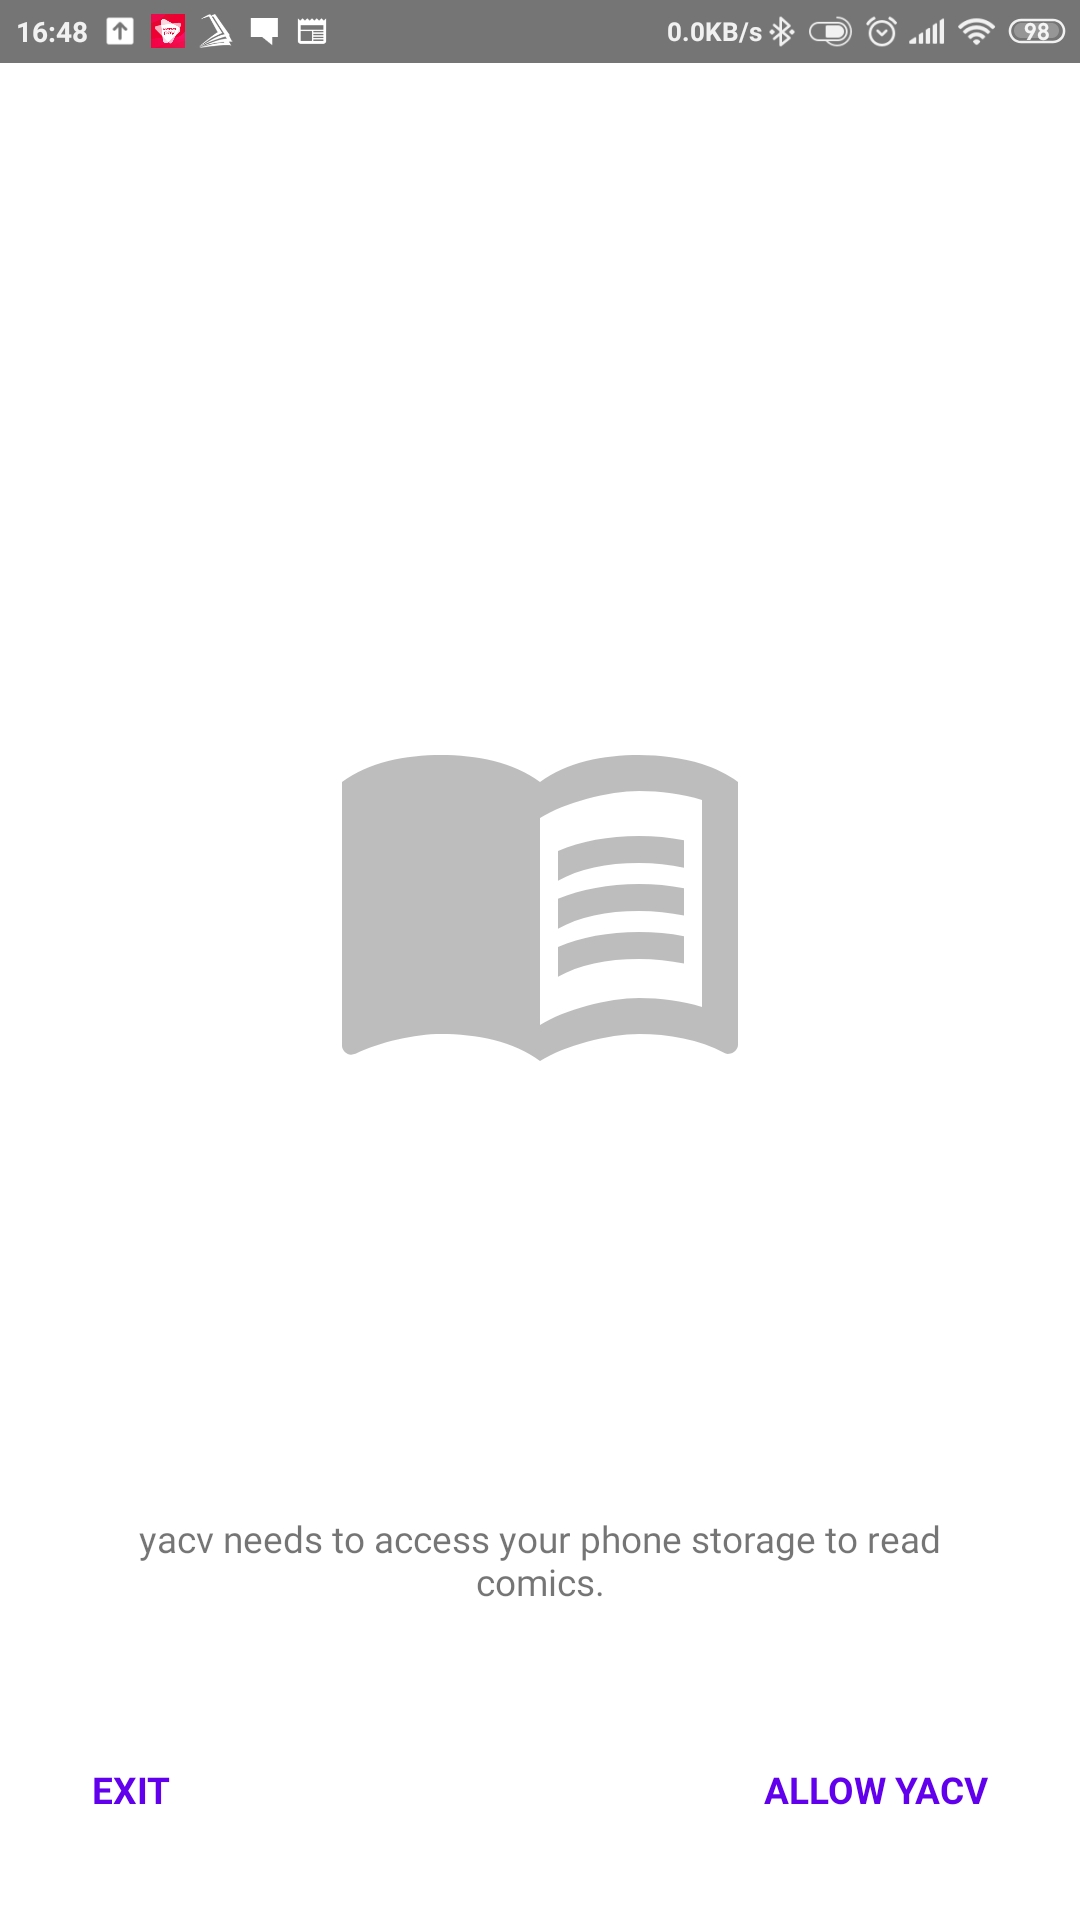
\includegraphics[scale=0.12]{../images/Screenshot_2021-05-25-08-05-43-397_com.uet.nvmnghia.yacv}
    \caption{Màn hình Quyền đọc}
    \label{fig:permission_screen}
\end{figure}

\subsection{Màn hình Duyệt truyện}

Hai màn hình - Màn hình Thư viện và Màn hình Thư mục dùng để duyệt danh sách
truyện. Màn hình Thư viện là màn hiển thị mặc định. Từ nó, khi ấn vào một thư
mục, ta truy cập được Màn hình Thư mục tương ứng.

\begin{figure}[H]
    \centering
    \begin{subfigure}[b]{0.328\textwidth}
        \centering
        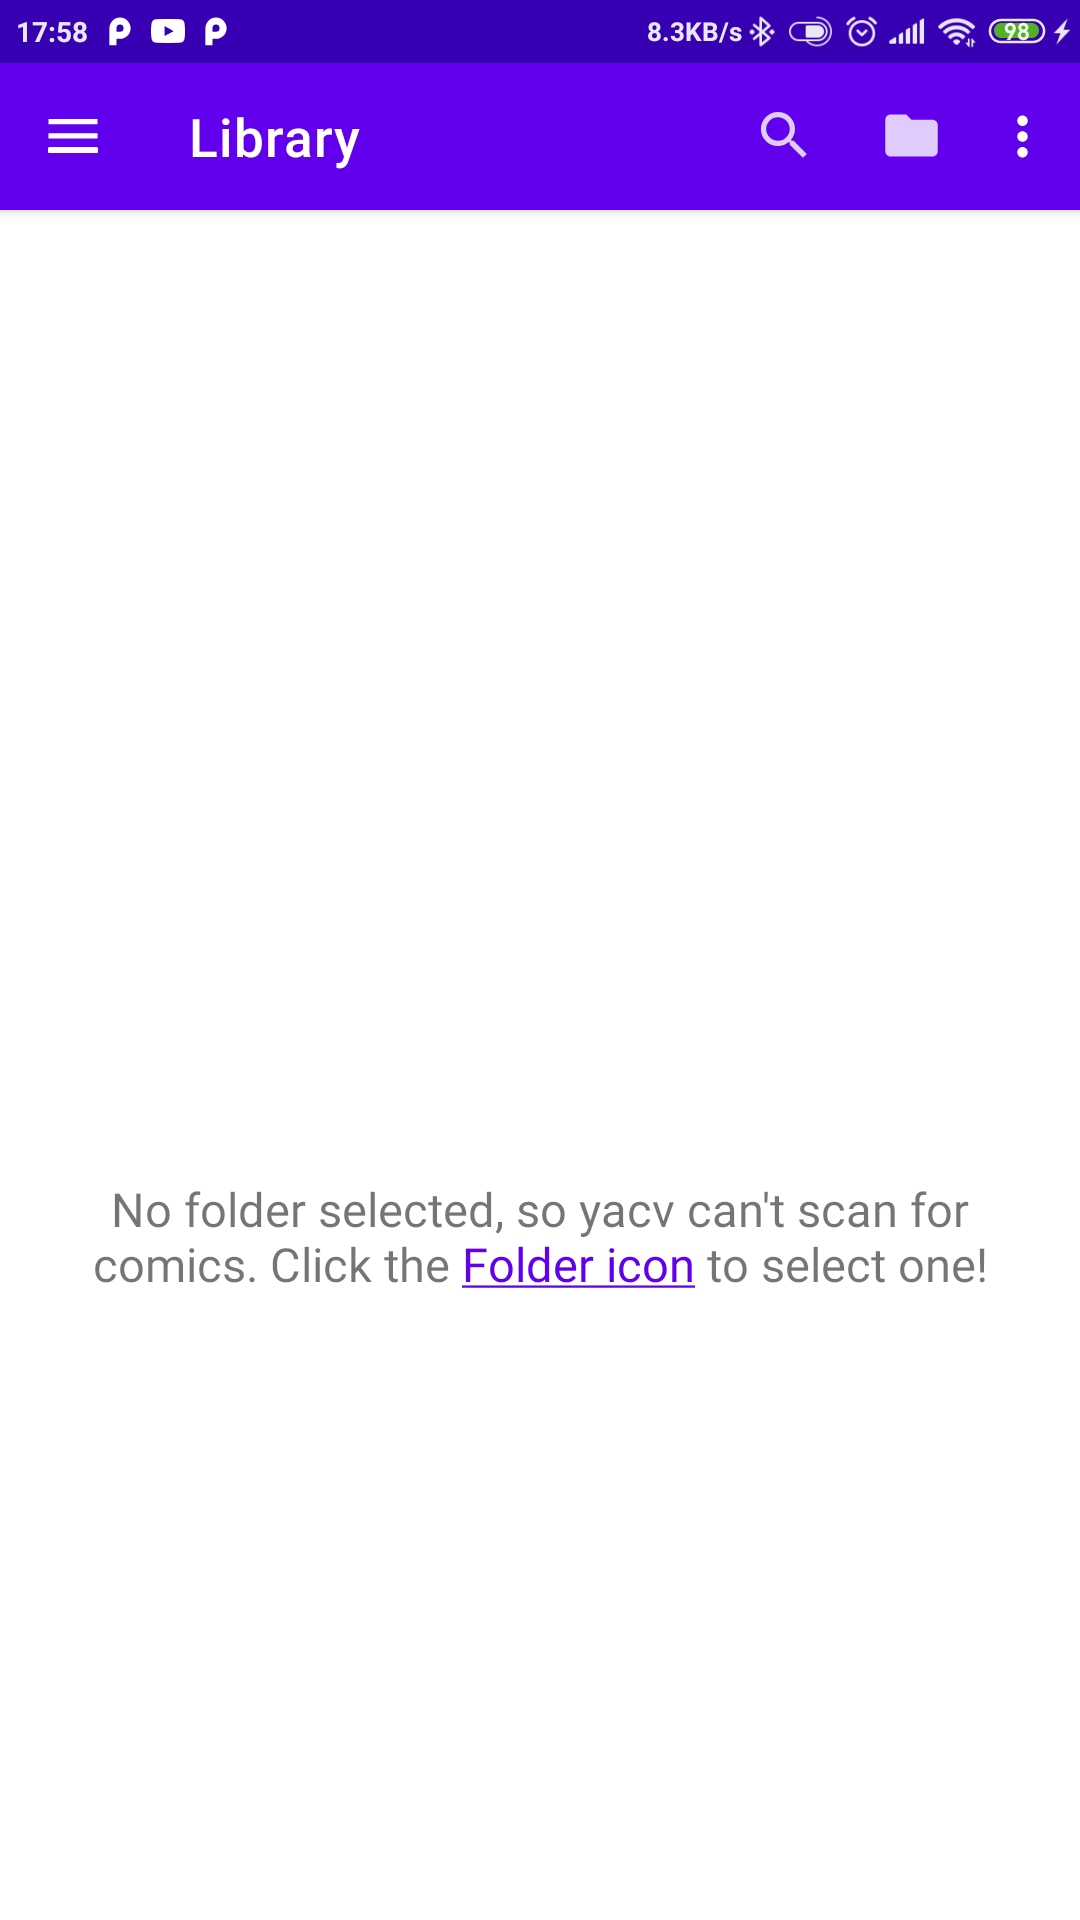
\includegraphics[scale=0.12]{../images/Screenshot_2021-05-27-17-58-36-567_com.uet.nvmnghia.yacv}
        \caption{Màn hình Thư viện trống}
        \label{fig:empty_library_screen}
    \end{subfigure}
    \hfill
    \begin{subfigure}[b]{0.328\textwidth}
        \centering
        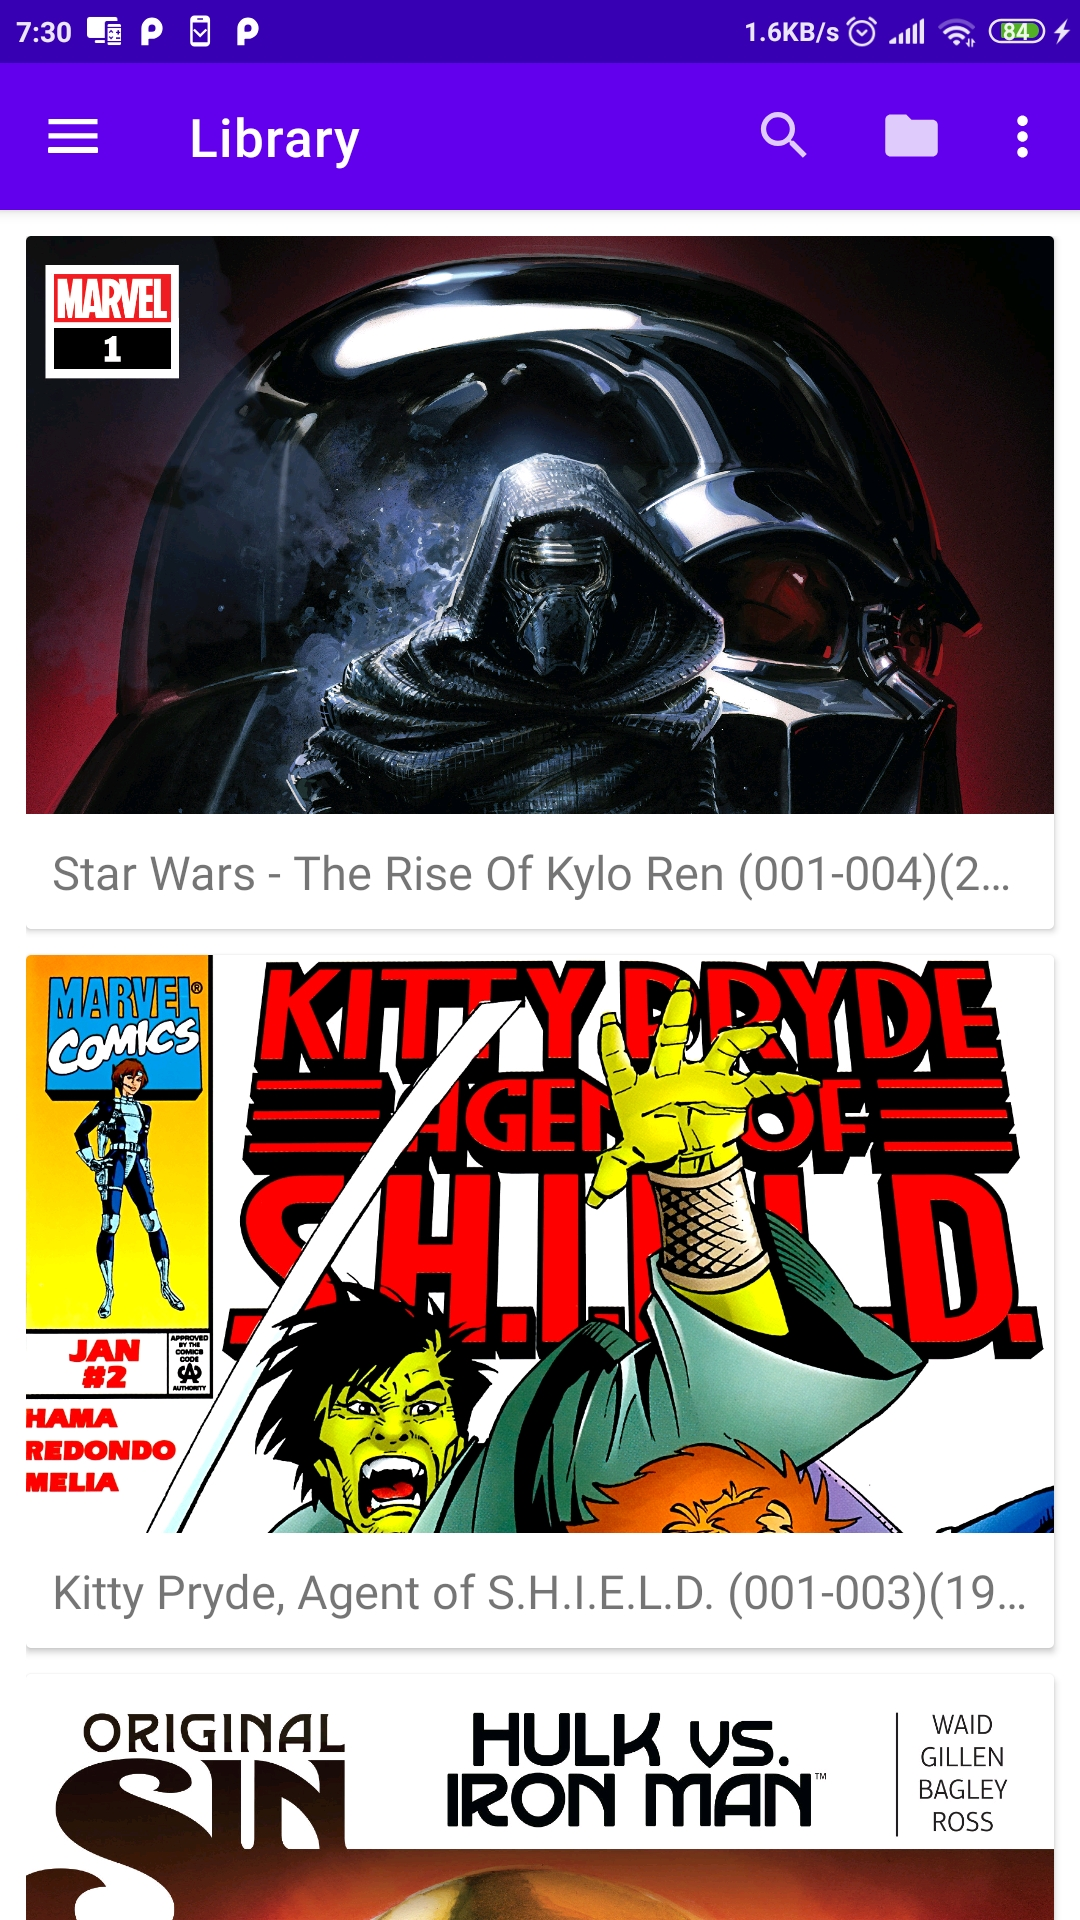
\includegraphics[scale=0.12]{../images/Screenshot_2021-05-25-07-30-21-599_com.uet.nvmnghia.yacv}
        \caption{Màn hình Thư viện}
        \label{fig:library_screen}
    \end{subfigure}
    \hfill
    \begin{subfigure}[b]{0.328\textwidth}
        \centering
        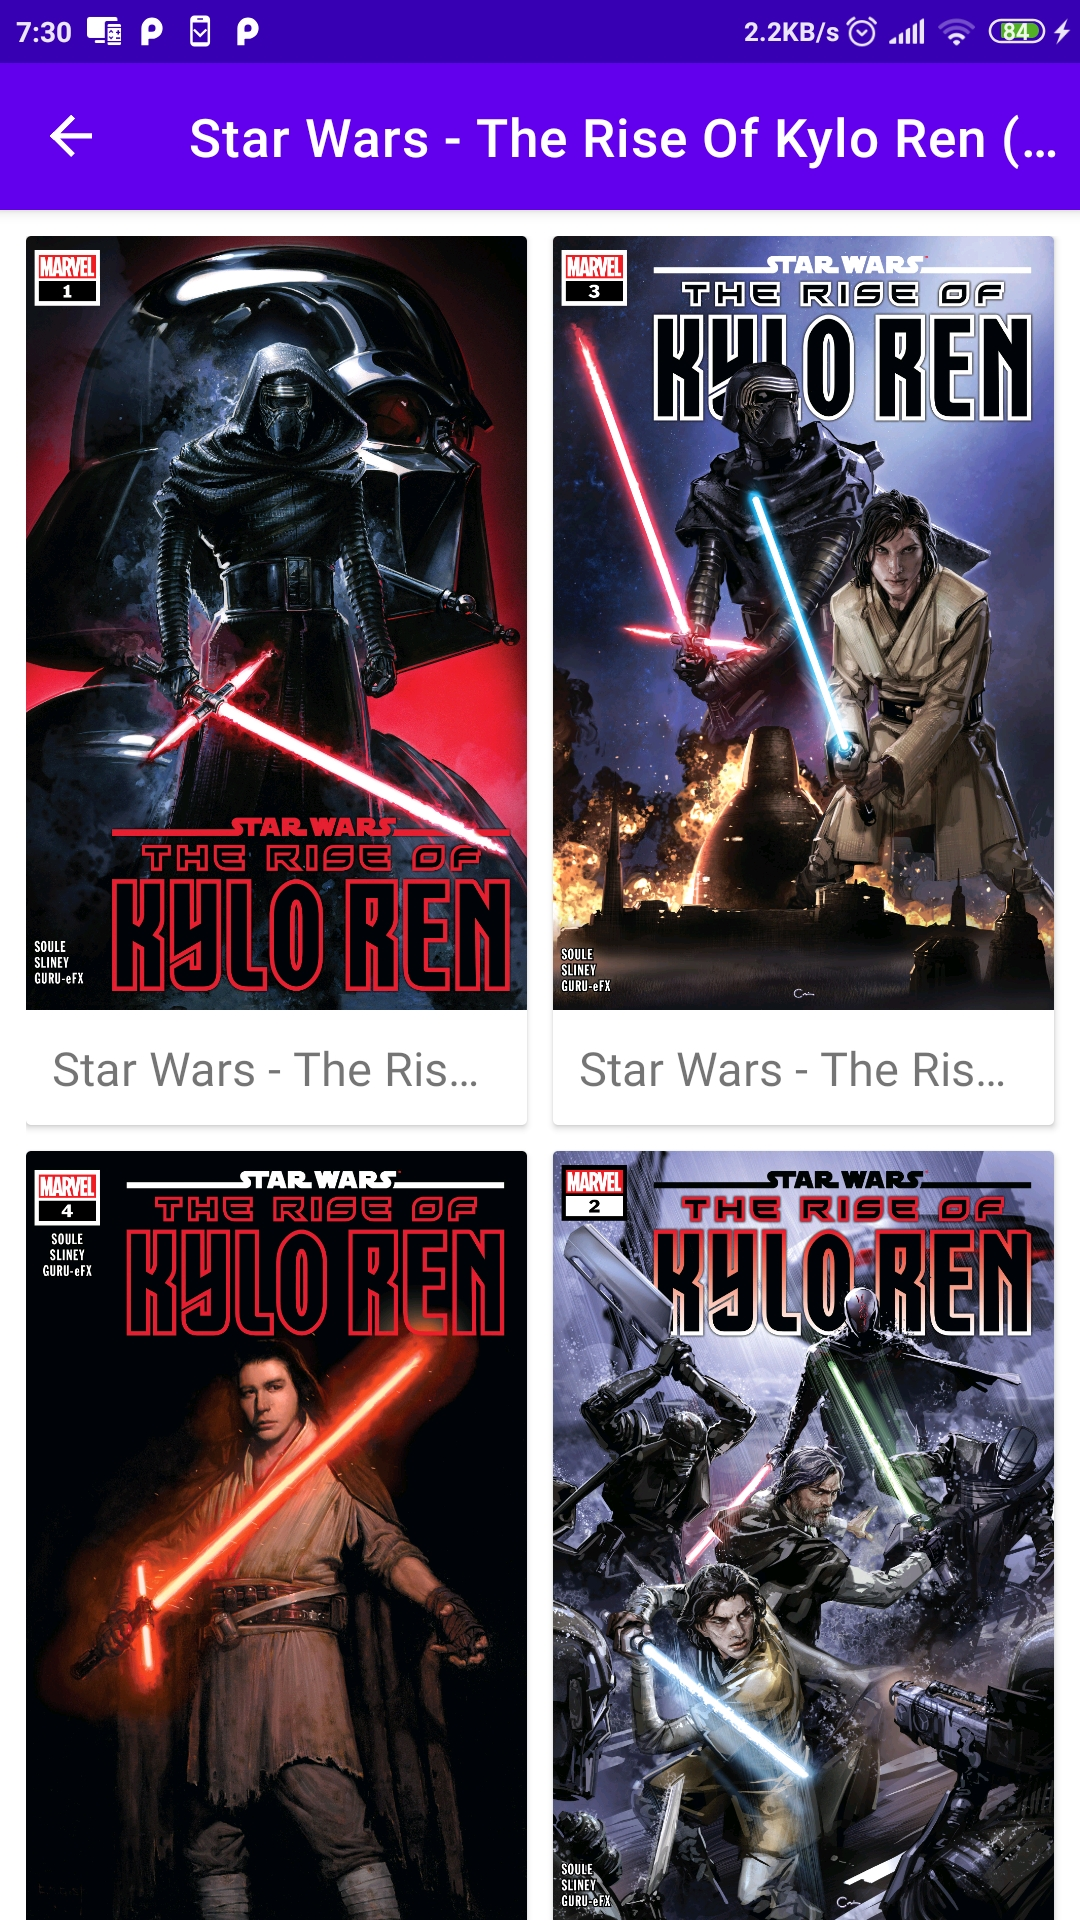
\includegraphics[scale=0.12]{../images/Screenshot_2021-05-25-07-30-42-216_com.uet.nvmnghia.yacv}
        \caption{Màn hình Thư mục}
        \label{fig:folder_screen}
    \end{subfigure}
    \caption{Hai Màn hình Duyệt truyện}
    \label{fig:2-browsing-screens}
\end{figure}

\subsection{Màn hình Đọc truyện}

Màn hình Đọc truyện dùng để xem các trang truyện, được truy cập bằng cách ấn vào
một truyện trong Màn hình Thư mục.

\begin{figure}[H]
    \centering
    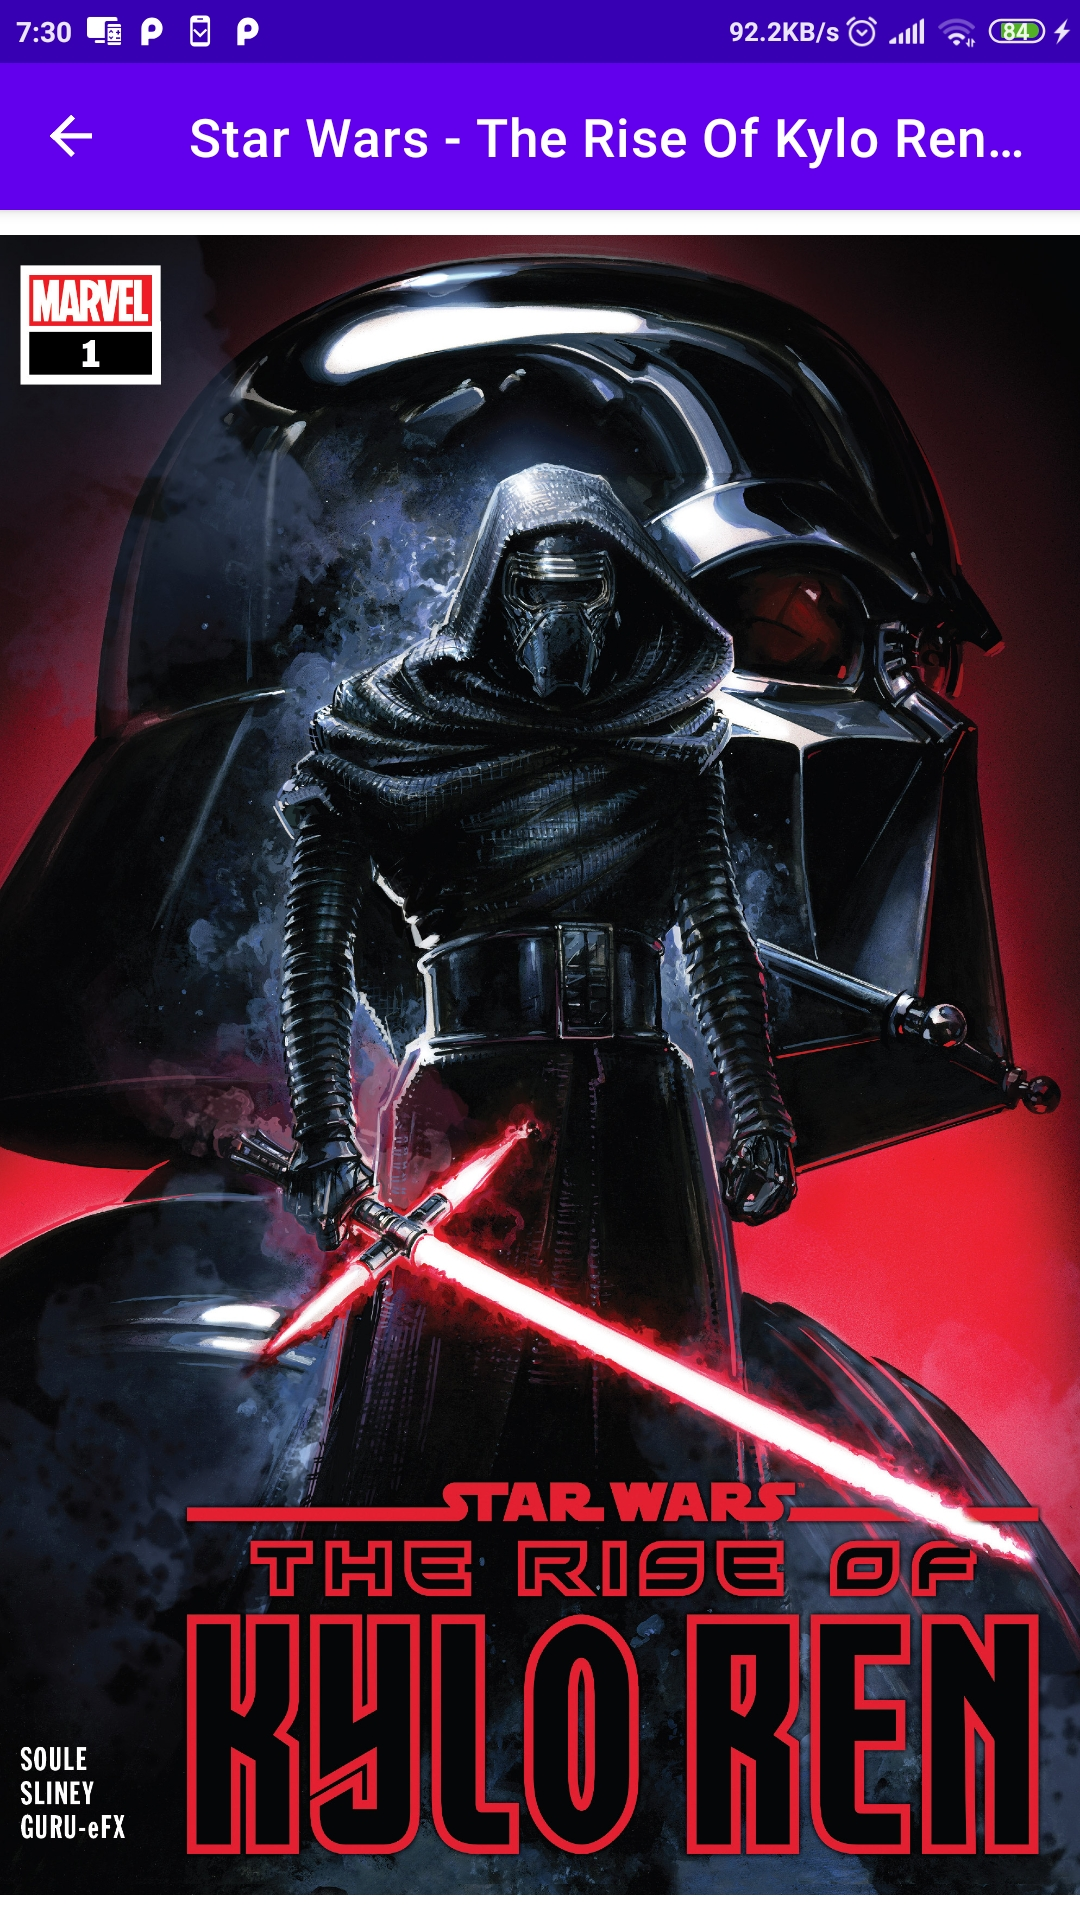
\includegraphics[scale=0.12]{../images/Screenshot_2021-05-25-07-30-56-357_com.uet.nvmnghia.yacv}
    \caption{Màn hình Đọc truyện}
    \label{fig:reader_screen}
\end{figure}

\subsection{Màn hình Metadata}

Màn hình này hiển thị metadata đi kèm, được truy cập từ Màn hình Đọc truyện.

\begin{figure}[H]
    \centering
    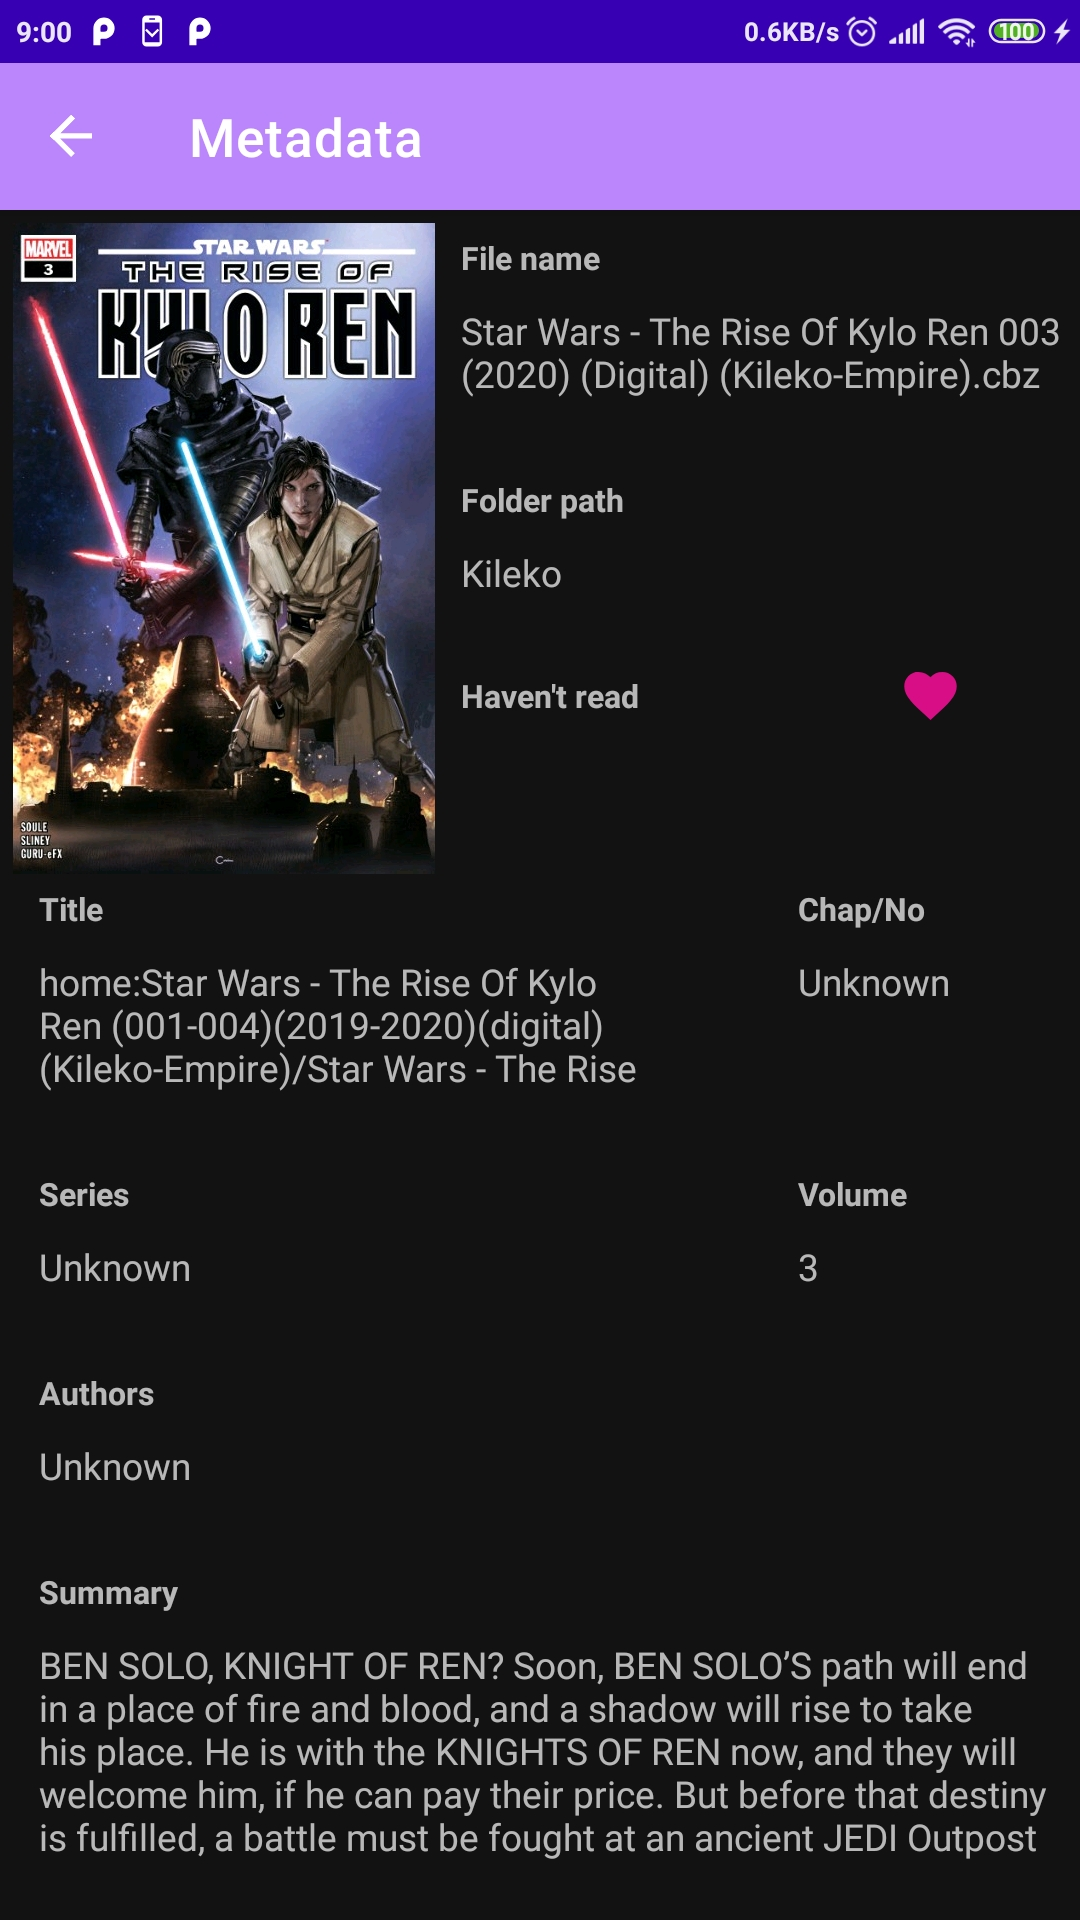
\includegraphics[scale=0.12]{../images/Screenshot_2021-05-17-09-00-17-548_com.uet.nvmnghia.yacv}
    \caption{Màn hình Metadata}
    \label{fig:metadata_screen}
\end{figure}

\subsection{Màn hình Tìm kiếm}

Màn hình Tìm kiếm gồm hai màn hình con gần giống nhau, dùng để rút gọn số lượng
kết quả hiển thị. Cả hai màn hình đều có đích đến là Màn hình Đọc truyện.

\begin{figure}[H]
    \centering
    \begin{subfigure}[b]{0.49\textwidth}
        \centering
        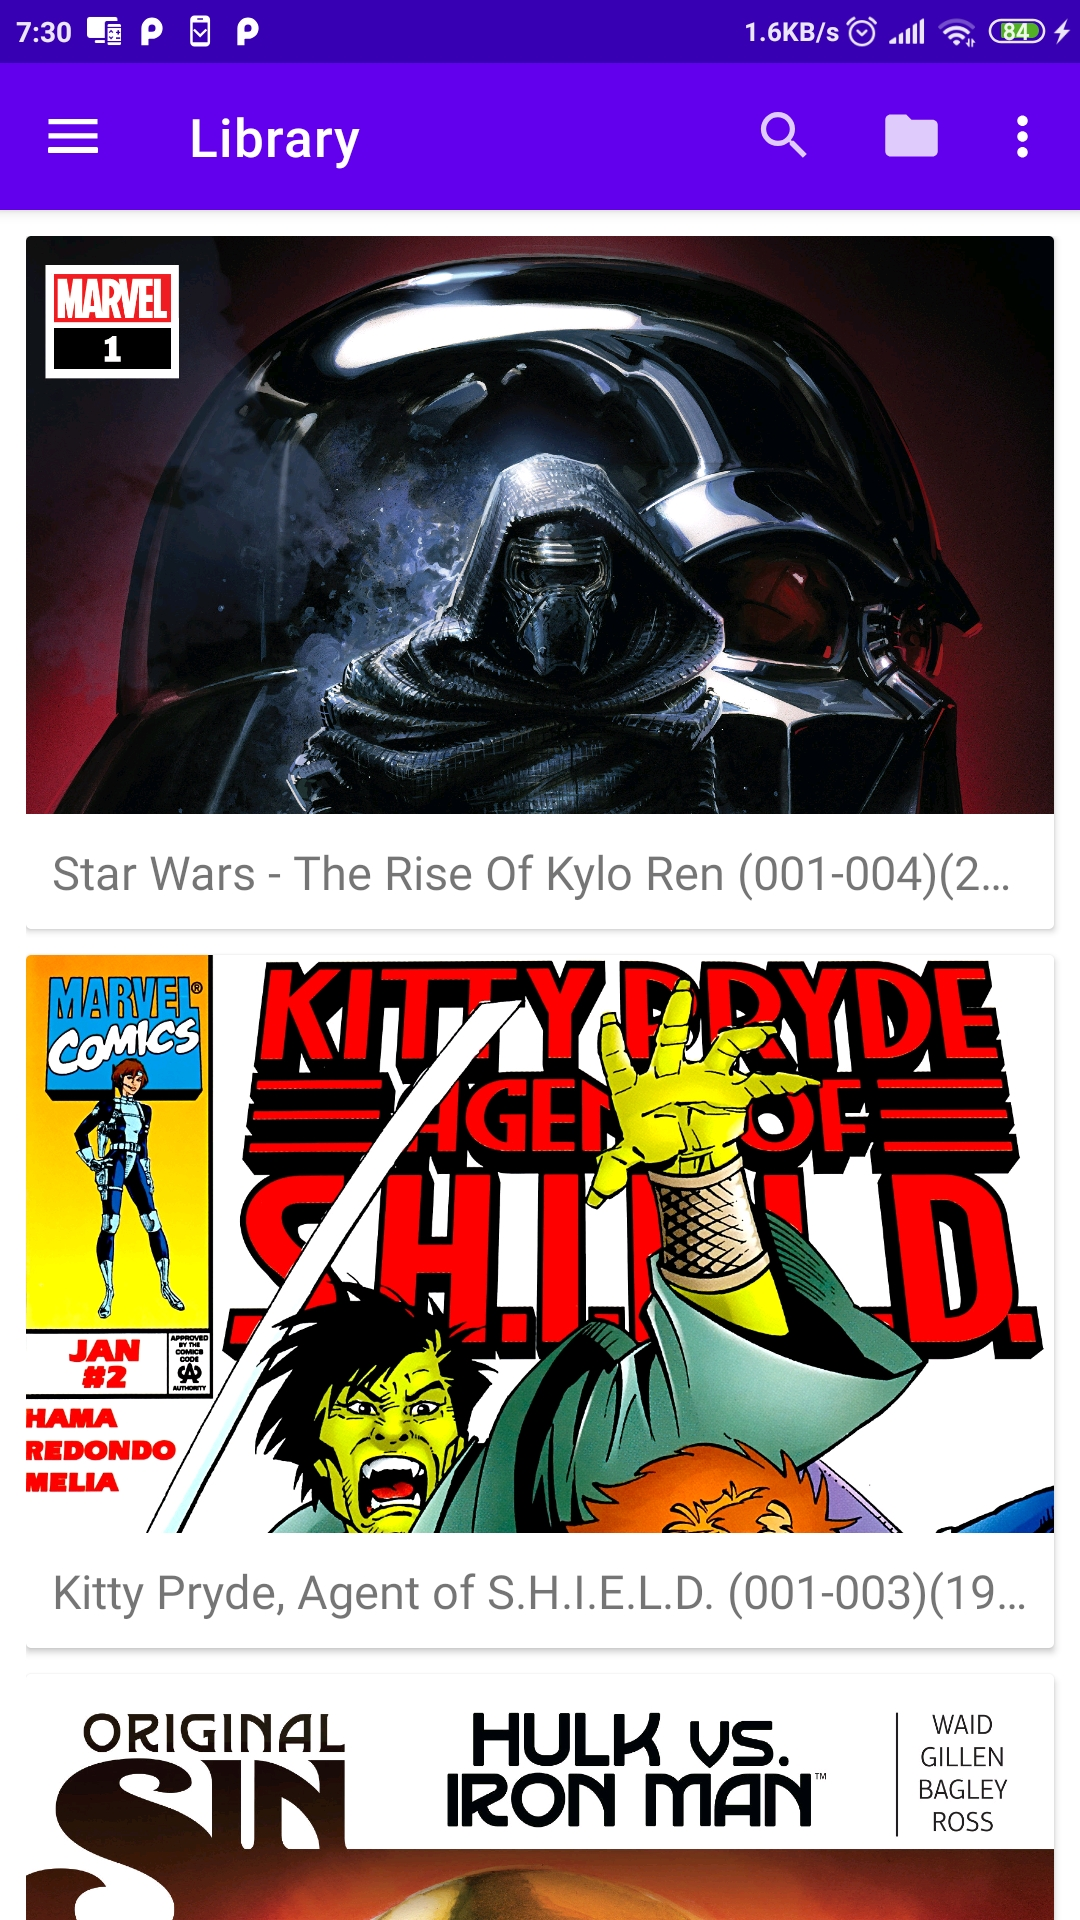
\includegraphics[scale=0.12]{../images/Screenshot_2021-05-25-07-30-21-599_com.uet.nvmnghia.yacv}
        \caption{Màn hình Tìm kiếm Tổng quan}
        \label{fig:search_overall_screen}
    \end{subfigure}
    \hfill
    \begin{subfigure}[b]{0.49\textwidth}
        \centering
        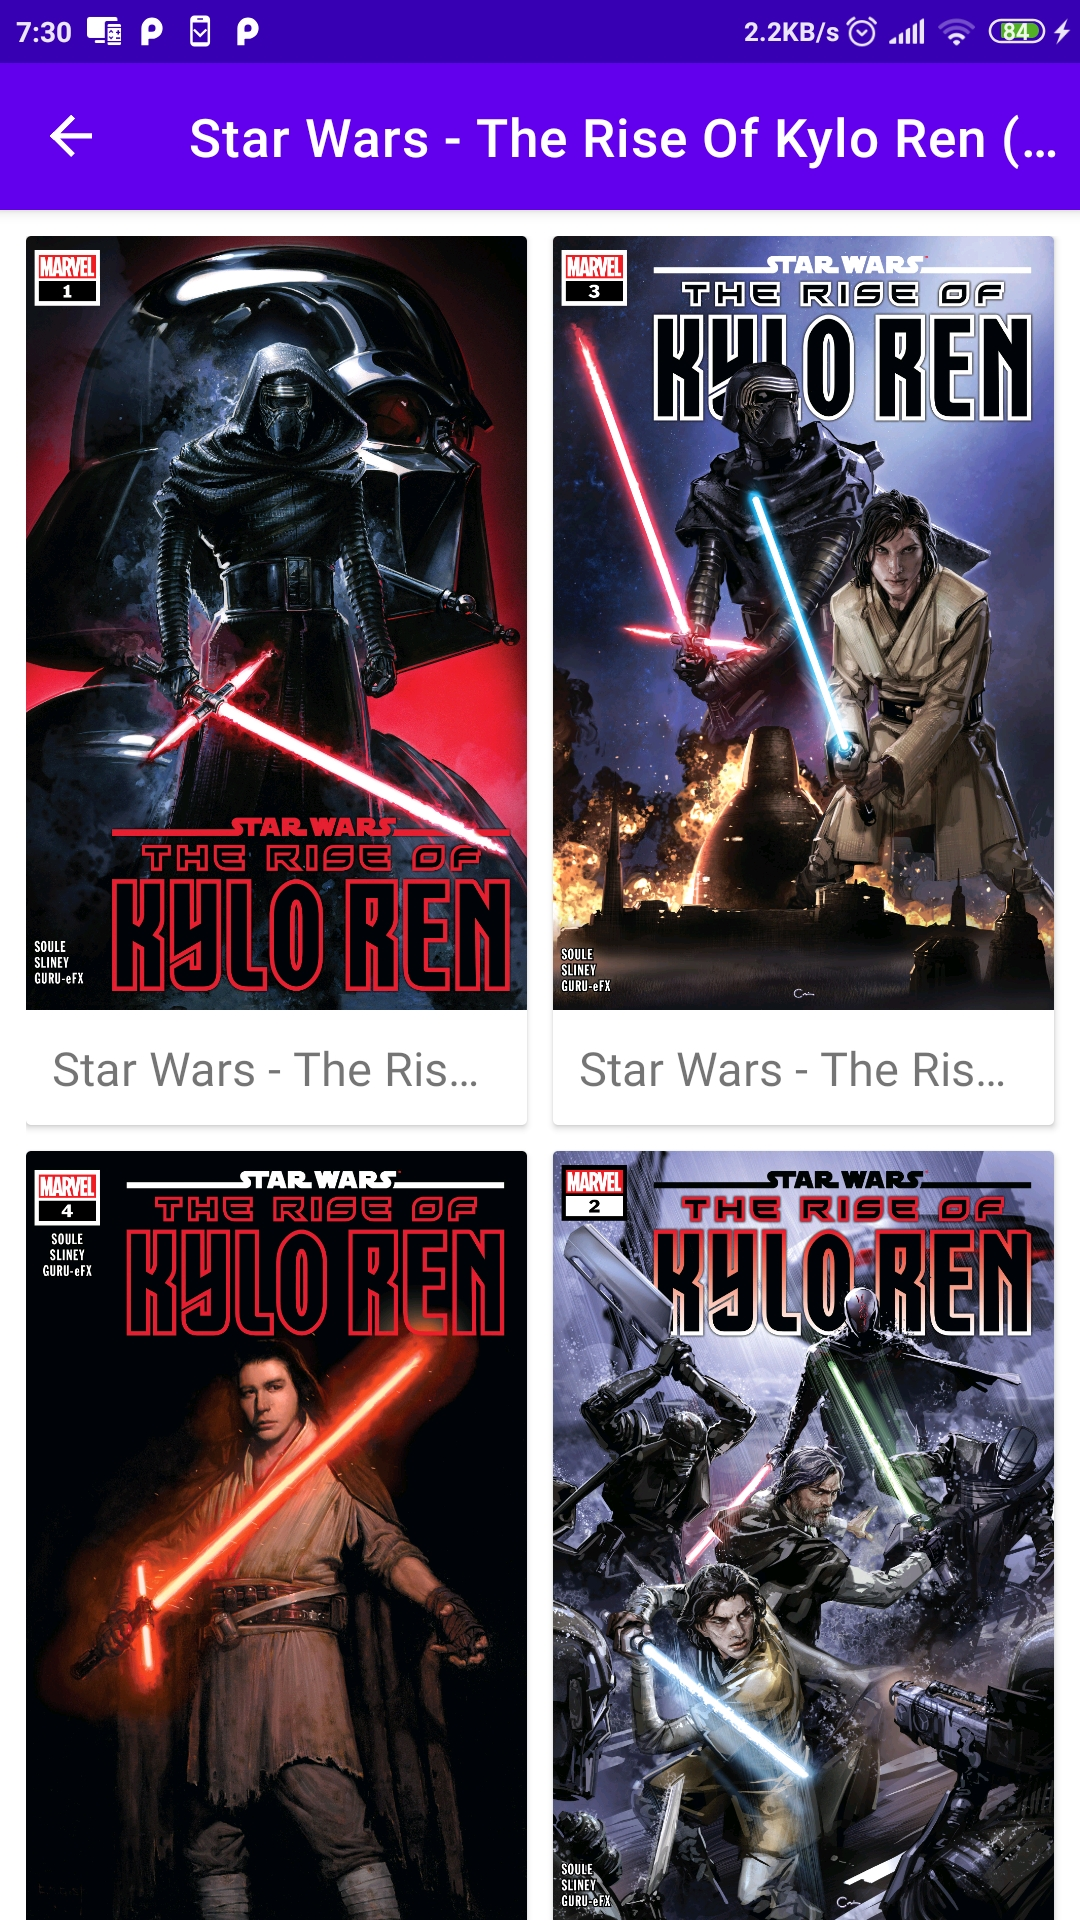
\includegraphics[scale=0.12]{../images/Screenshot_2021-05-25-07-30-42-216_com.uet.nvmnghia.yacv}
        \caption{Màn hình Tìm kiếm Chi tiết}
        \label{fig:search_detail_screen}
    \end{subfigure}
    \caption{Hai Màn hình Tìm kiếm}
    \label{fig:2-searching-screens}
\end{figure}

\end{document}
